\section{PCA 主成分分析}

\begin{definition}[主成分分析]
    主成分分析可以用较少的新变量替换原来较多的新变量，而且是这些较少的新变量尽可能多地保留原来所反映的信息。

    主成分分析是数据降维算法的一种，降维是将高维度的数据（指标太多）保留下最重要的一些特征，去除噪声和不重要的特征.
\end{definition}

\begin{warning}
    \begin{itemize}
        \item 主成分分析的困难在于要能够给出主成分的较好解释，所提取的主成分中如有一个主成分解释不了，整个主成分分析也就失败了。
        \item \textcolor{purple}{主成分分析不可用于评价类模型}。
        \item 主成分分析可用于聚类分析，将自变量进行降维方便画图。
        \item 主成分分析也可用于回归分析解决多重共线性的问题。
    \end{itemize}
\end{warning}

\begin{theorem}[主成分分析的思想]
    假设有 $n$ 个样本， $p$ 个指标，则可构成大小为 $\mathrm{n} \times \mathrm{p}$ 的样本矩阵 $x$ ：
    $$
        \mathrm{X}=\left[\begin{array}{cccc}
                \mathrm{x}_{11}           & \mathrm{x}_{12}           & \cdots & \mathrm{x}_{1 \mathrm{p}} \\
                \mathrm{x}_{21}           & \mathrm{x}_{22}           & \cdots & \mathrm{x}_{2 \mathrm{p}} \\
                \vdots                    & \vdots                    & \ddots & \vdots                    \\
                \mathrm{x}_{\mathrm{n} 1} & \mathrm{x}_{\mathrm{n} 2} & \cdots & \mathrm{x}_{\mathrm{np}}
            \end{array}\right]=\left(\mathrm{x}_1, \mathrm{x}_2, \cdots, \mathrm{x}_{\mathrm{p}}\right)
    $$

    假设我们想找到新的一组变量 $\mathrm{z}_1, \mathrm{z}_2, \ldots, \mathrm{z}_{\mathrm{m}}(\mathrm{m} \leq \mathrm{p})$ ，且它们满足：
    $$
        \left\{\begin{array}{l}
            \mathrm{z}_1=\mathrm{l}_{11} \mathrm{x}_1+\mathrm{l}_{12} \mathrm{x}_2+\cdots+\mathrm{l}_{1 \mathrm{p}} \mathrm{x}_{\mathrm{p}} \\
            \mathrm{z}_2=\mathrm{l}_{21} \mathrm{x}_1+\mathrm{l}_{22} \mathrm{x}_2+\cdots+\mathrm{l}_{2 \mathrm{p}} \mathrm{x}_{\mathrm{p}} \\
            \cdots                                                                                                                          \\
            \mathrm{z}_{\mathrm{m}}=\mathrm{l}_{\mathrm{m} 1} \mathrm{x}_1+\mathrm{l}_{\mathrm{m} 2} \mathrm{x}_2+\cdots+\mathrm{l}_{\mathrm{mp}} \mathrm{x}_{\mathrm{p}}
        \end{array}\right.
    $$

    系数 $l_{\mathrm{ij}}$ 的确定原则：
    \begin{itemize}
        \item 1．$z_i$ 与 $z_j(i \neq j ; i, j=1,2, \ldots, m)$ 相互无关；
        \item 2． $\mathrm{z}_1$ 是 $\mathrm{x}_1, \mathrm{x}_2, \ldots, \mathrm{x}_{\mathrm{p}}$ 的一切线性组合中方差最大者；
        \item 3．$z_2$ 是与 $z_1$ 不相关的 $x_1, x_2, \ldots, x_p$ 的所有线性组合中方差最大者；
        \item 4．以此类推， $\mathrm{z}_{\mathrm{m}}$ 是与 $\mathrm{z}_1, \mathrm{z}_2, \ldots, \mathrm{z}_{\mathrm{m}-1}$ 不相关的 $\mathrm{x}_1, \mathrm{x}_2, \ldots, \mathrm{x}_{\mathrm{p}}$ 的所有线性组合中方差最大者；
        \item 5．新变量指标 $z_1, z_2, \ldots, z_m$ 分别称为原变量指标 $x_1, x_2, \ldots, x_p$ 的第一，第二，$\ldots$ ，第 $m$ 主成分。
    \end{itemize}
\end{theorem}

\subsection{PCA 降维的操作流程}

\begin{warning}
    并非所有的数据都适用于主成分分析的。主成分分析本身并不是目的，实际应用中主成分分析往往是一种手段。目的是通过主成分分析简化数据结构，在此基础上进行进一步的分析。

    主成分分析使用前，需要判断变量之间是否存在强相关性，或者说多重共线性，检测的方法有很多，例如：
    \begin{itemize}
        \item 相关性矩阵 (Correlation Matrix)
        \item KMO检验 (Kaiser-Meyer-Olkin Test)
        \item Bartlett's 球形检验 (Bartlett's Test of Sphericity)
        \item 方差膨胀因子 (Variance Inflation Factor, VIF)
    \end{itemize}
\end{warning}

\begin{definition}[KMO 检验]
    KMO 检验通过比较变量间的简单相关系数和偏相关系数，来检验数据的"纯度"。其核心思想是：如果变量之间存在共同的潜在因子（主成分），那么它们之间的简单相关性应该远大于偏相关性（即在控制了其他变量后，两个变量之间的相关性应该很小）。
    KMO 统计量的计算公式为：
    \begin{equation}
        \text{KMO} = \frac{\displaystyle\sum_{i \neq j} r_{ij}^2}{\displaystyle\sum_{i \neq j} r_{ij}^2 + \sum_{i \neq j} a_{ij}^2}
    \end{equation}
    其中，$r_{ij}$ 是变量 $i$ 和 $j$ 之间的简单相关系数，$a_{ij}$ 是在控制了其他所有变量后，变量 $i$ 和 $j$ 之间的偏相关系数。

    KMO 的取值范围在 $0$ 到 $1$ 之间。值越接近 $1$，说明变量间的共同因素越多，数据越适合进行主成分分析。\\
    Kaiser (1974) 给出的判断标准如下：
    \begin{table}[H]
        \centering
        \begin{tabular}{ccccccc}
            \toprule
            \textbf{KMO值范围} & 0.90以上 & 0.80-0.89 & 0.70-0.79 & 0.60-0.69 & 0.50-0.59 & 0.50以下 \\
            \midrule
            \textbf{适合程度}   & 非常适合   & 很适合       & 适合        & 一般        & 不佳        & 不适合    \\
            \bottomrule
        \end{tabular}
    \end{table}
\end{definition}

\begin{definition}[Bartlett's 球形检验]
    Bartlett's 检验是一种统计假设检验，用于判断相关性矩阵是否为一个单位矩阵（即对角线为1，其余为0）。如果相关性矩阵是单位矩阵，则说明所有变量都是相互独立的，不适合进行主成分分析。

    我们进行假设：
    \begin{itemize}
        \item \textbf{原假设 ($H_0$)}: 相关性矩阵 $\mathbf{R}$ 是一个单位矩阵 ($\mathbf{R} = \mathbf{I}$)。
        \item \textbf{备择假设 ($H_1$)}: 相关性矩阵 $\mathbf{R}$ 不是一个单位矩阵。
    \end{itemize}

    检验统计量近似服从卡方 ($\chi^2$) 分布，其计算公式为：
    \begin{equation}
        \chi^2 = -\left(n - 1 - \frac{2p + 5}{6}\right) \ln(|\mathbf{R}|)
    \end{equation}
    其中：$n$ 是样本数量，$p$ 是变量数量，$|\mathbf{R}|$ 是相关性矩阵 $\mathbf{R}$ 的行列式。
    该统计量的自由度为 $df = \frac{p(p-1)}{2}$。

    计算出统计量后，我们可以得到一个对应的 $p$ 值。如果 $p$ 值非常小（例如 $p < 0.05$），我们就可以拒绝原假设 $H_0$，认为变量之间存在显著的相关性，因此数据适合进行主成分分析。

    \begin{tips}
        做因子分析时是一样的，如果该值较大，且其对应的相伴概率值小于用户心中的显著性水平，那么应该拒绝零假设，认为相关系数不可能是单位阵，即原始变量之间存在相关性，适合于作因子分析。相反不适合作因子分析。
    \end{tips}
\end{definition}

\begin{lstlisting}[style=python]
Compute the Bartlett sphericity test.
H0: The matrix of population correlations is equal to I. H1: The matrix of population correlations is not equal to I.
The formula for Bartlett's Sphericity test is:
-1*(n-1-((2p+5)/6))*ln(det(R))
Where R det(R) is the determinant of the correlation matrix, and p is the number of variables.
\end{lstlisting}

\begin{definition}[方差膨胀因子]
    VIF 是衡量多重共线性严重程度的指标。虽然它常用于回归分析的诊断，但其原理可以直接用于判断 PCA 的适用性，因为它直接度量了一个变量在多大程度上能被其他变量所解释。
    对于第 $j$ 个变量 $X_j$，其 VIF 值的计算步骤如下：
    \begin{enumerate}
        \item 构建一个线性回归模型，其中 $X_j$ 是因变量，所有其他 $p-1$ 个变量是自变量：
              $$ X_j = \beta_0 + \beta_1 X_1 + \dots + \beta_{j-1} X_{j-1} + \beta_{j+1} X_{j+1} + \dots + \beta_p X_p + \epsilon $$
        \item 计算这个回归模型的决定系数 $R_j^2$。$R_j^2$ 表示其他变量能解释 $X_j$ 方差的比例。
        \item 第 $j$ 个变量的 VIF 值定义为：
              \begin{equation}
                  \text{VIF}_j = \frac{1}{1 - R_j^2}
              \end{equation}
    \end{enumerate}

    VIF 的值越大，说明变量 $X_j$ 与其他变量的共线性越强。
    \begin{itemize}
        \item VIF = 1: 不存在多重共线性
        \item 1 < VIF < 5: 存在一定的共线性，但通常可以接受
        \item VIF $\ge$ 5 或 10: 存在严重的共线性
    \end{itemize}
    在 PCA 的前置检验中，我们期望看到一些较大的 VIF 值，这恰恰说明了变量间存在冗余信息，可以通过 PCA 进行有效合并和降维。
\end{definition}

以上检验均可以直接调库实现。

\begin{lstlisting}[style=python]
print("--- 1. 相关性矩阵检验 ---")
corr_matrix = df_features.corr()
plt.figure(figsize=(8, 6))
sns.heatmap(corr_matrix, annot=True, cmap='coolwarm', fmt=".2f")
plt.title('特征相关性矩阵热力图')
plt.show()

print("--- 2. KMO 检验 ---")
kmo_all, kmo_model = calculate_kmo(df_features)

print("--- 3. Bartlett's 球形检验 ---")
chi_square_value, p_value = calculate_bartlett_sphericity(df_features)

print("--- 4. 方差膨胀因子 (VIF) 检验 ---")
X_vif = sm.add_constant(df_features)
vif_data = pd.DataFrame()
vif_data["feature"] = X_vif.columns
vif_data["VIF"] = [variance_inflation_factor(X_vif.values, i) for i in range(X_vif.shape[1])]
\end{lstlisting}

\begin{table}[H]
    \centering
    \caption{客户信用评级数据 (保留两位小数)}
    \label{tab:customer_data}
    \begin{tabular}{@{}cccccc@{}}
        \toprule
        \textbf{客户编号} & \textbf{能力} & \textbf{品格} & \textbf{担保} & \textbf{资本} & \textbf{环境} \\ \midrule
        1             & 61.76       & 60.82       & 62.72       & 61.39       & 63.88       \\
        2             & 65.26       & 65.98       & 65.97       & 66.52       & 65.37       \\
        3             & 63.19       & 64.81       & 65.06       & 62.85       & 65.10       \\
        4             & 65.02       & 63.93       & 64.31       & 64.04       & 62.36       \\
        5             & 64.23       & 65.44       & 64.01       & 62.93       & 65.47       \\
        6             & 65.84       & 64.00       & 65.10       & 64.69       & 64.97       \\
        7             & 64.85       & 62.85       & 62.75       & 64.71       & 64.24       \\
        8             & 56.94       & 58.12       & 62.72       & 59.12       & 65.57       \\
        9             & 66.88       & 68.81       & 65.50       & 67.83       & 64.48       \\
        10            & 61.22       & 61.13       & 62.10       & 61.64       & 63.45       \\
        11            & 63.89       & 65.23       & 63.05       & 62.98       & 63.38       \\
        12            & 3.92        & 63.05       & 62.98       & 63.35       & 63.81       \\ \bottomrule
    \end{tabular}
\end{table}

\subsubsection{数据标准化}

为了消除不同特征的量纲和数值范围的影响，首先需要对数据进行标准化。其计算公式如下：
\[
    z_{ij} = \frac{x_{ij} - \bar{x}_j}{S_j},
    \qquad \text{其中，} \bar{x}_j = \frac{1}{n} \sum_{i=1}^{n} x_{ij},
    \quad S_j = \sqrt{\frac{\sum_{i=1}^{n} (x_{ij} - \bar{x}_j)^2}{n-1}}
\]

\subsubsection{计算相关系数矩阵}

计算标准化后的数据矩阵 $\mathbf{Z}$ 的相关系数矩阵 $\mathbf{R}$。（如果未进行标准化，则计算协方差矩阵 $\Sigma$）。再求解相关系数矩阵的特征值和特征向量：
\[
    \mathbf{R} = \frac{1}{n-1} Z^T Z
\]

求解满足以下方程的 $\lambda$ 和 $\mathbf{w}$：
\[
    \mathbf{R} \mathbf{w} = \lambda \mathbf{w}
\]
对于一个 $p \times p$ 的矩阵 $\mathbf{R}$，我们可以解出 $p$ 个特征值 $\lambda_1, \lambda_2, \ldots, \lambda_p$ 和与之对应的 $p$ 个特征向量 $\mathbf{w}_1, \mathbf{w}_2, \ldots, \mathbf{w}_p$。
我们将特征值从大到小排序：$\lambda_1 \ge \lambda_2 \ge \ldots \ge \lambda_p \ge 0$。
\begin{itemize}
    \item \textbf{特征值 ($\lambda_i$)}：代表了第 $i$ 个主成分能够解释的方差大小。$\lambda_1$ 最大，第一主成分解释了最多的数据方差。
\end{itemize}

\subsubsection{选择主成分}

我们希望用 $k$ 个主成分 ($k < p$) 来代替原来的 $p$ 个特征。如何确定 $k$ 的值？通常通过计算累计方差贡献率决定。
则第 $i$ 个主成分的方差贡献率为：
\[
    \text{Variance Explained}_i = \frac{\lambda_i}{\sum_{j=1}^p \lambda_j}
\]
选择最小的 $k$ 值，使得累计贡献率达到一个阈值（例如85\%或90\%）：
\[
    \sum_{i=1}^k \frac{\lambda_i}{\sum_{j=1}^p \lambda_j} \ge \text{Threshold (e.g., 0.85)}
\]

\begin{tips}
    对于某个主成分而言，指标前面的系数越大，代表该指标对该主成分的影响越大。
\end{tips}

\subsubsection{生成新的数据矩阵}

选定了前 $k$ 个主成分后，我们将这 $k$ 个对应的特征向量 $\mathbf{w}_1, \ldots, \mathbf{w}_k$ 按列组合成一个\textbf{投影矩阵} $W$：
\[
    W = \begin{pmatrix} \mathbf{w}_1 & \mathbf{w}_2 & \cdots & \mathbf{w}_k \end{pmatrix}_{p \times k}
\]
最后，将标准化后的原始数据矩阵 $Z$ 投影到这个新的坐标系上，得到降维后的新数据矩阵 $Y$：
\[
    Y = ZW
\]
这个新的矩阵 $Y$ 的维度是 $n \times k$，成功地将数据的特征从 $p$ 维降到了 $k$ 维。矩阵 $Y$ 中的每一列就是一个主成分的得分（Scores）。

\begin{figure} [H]
    \centering
    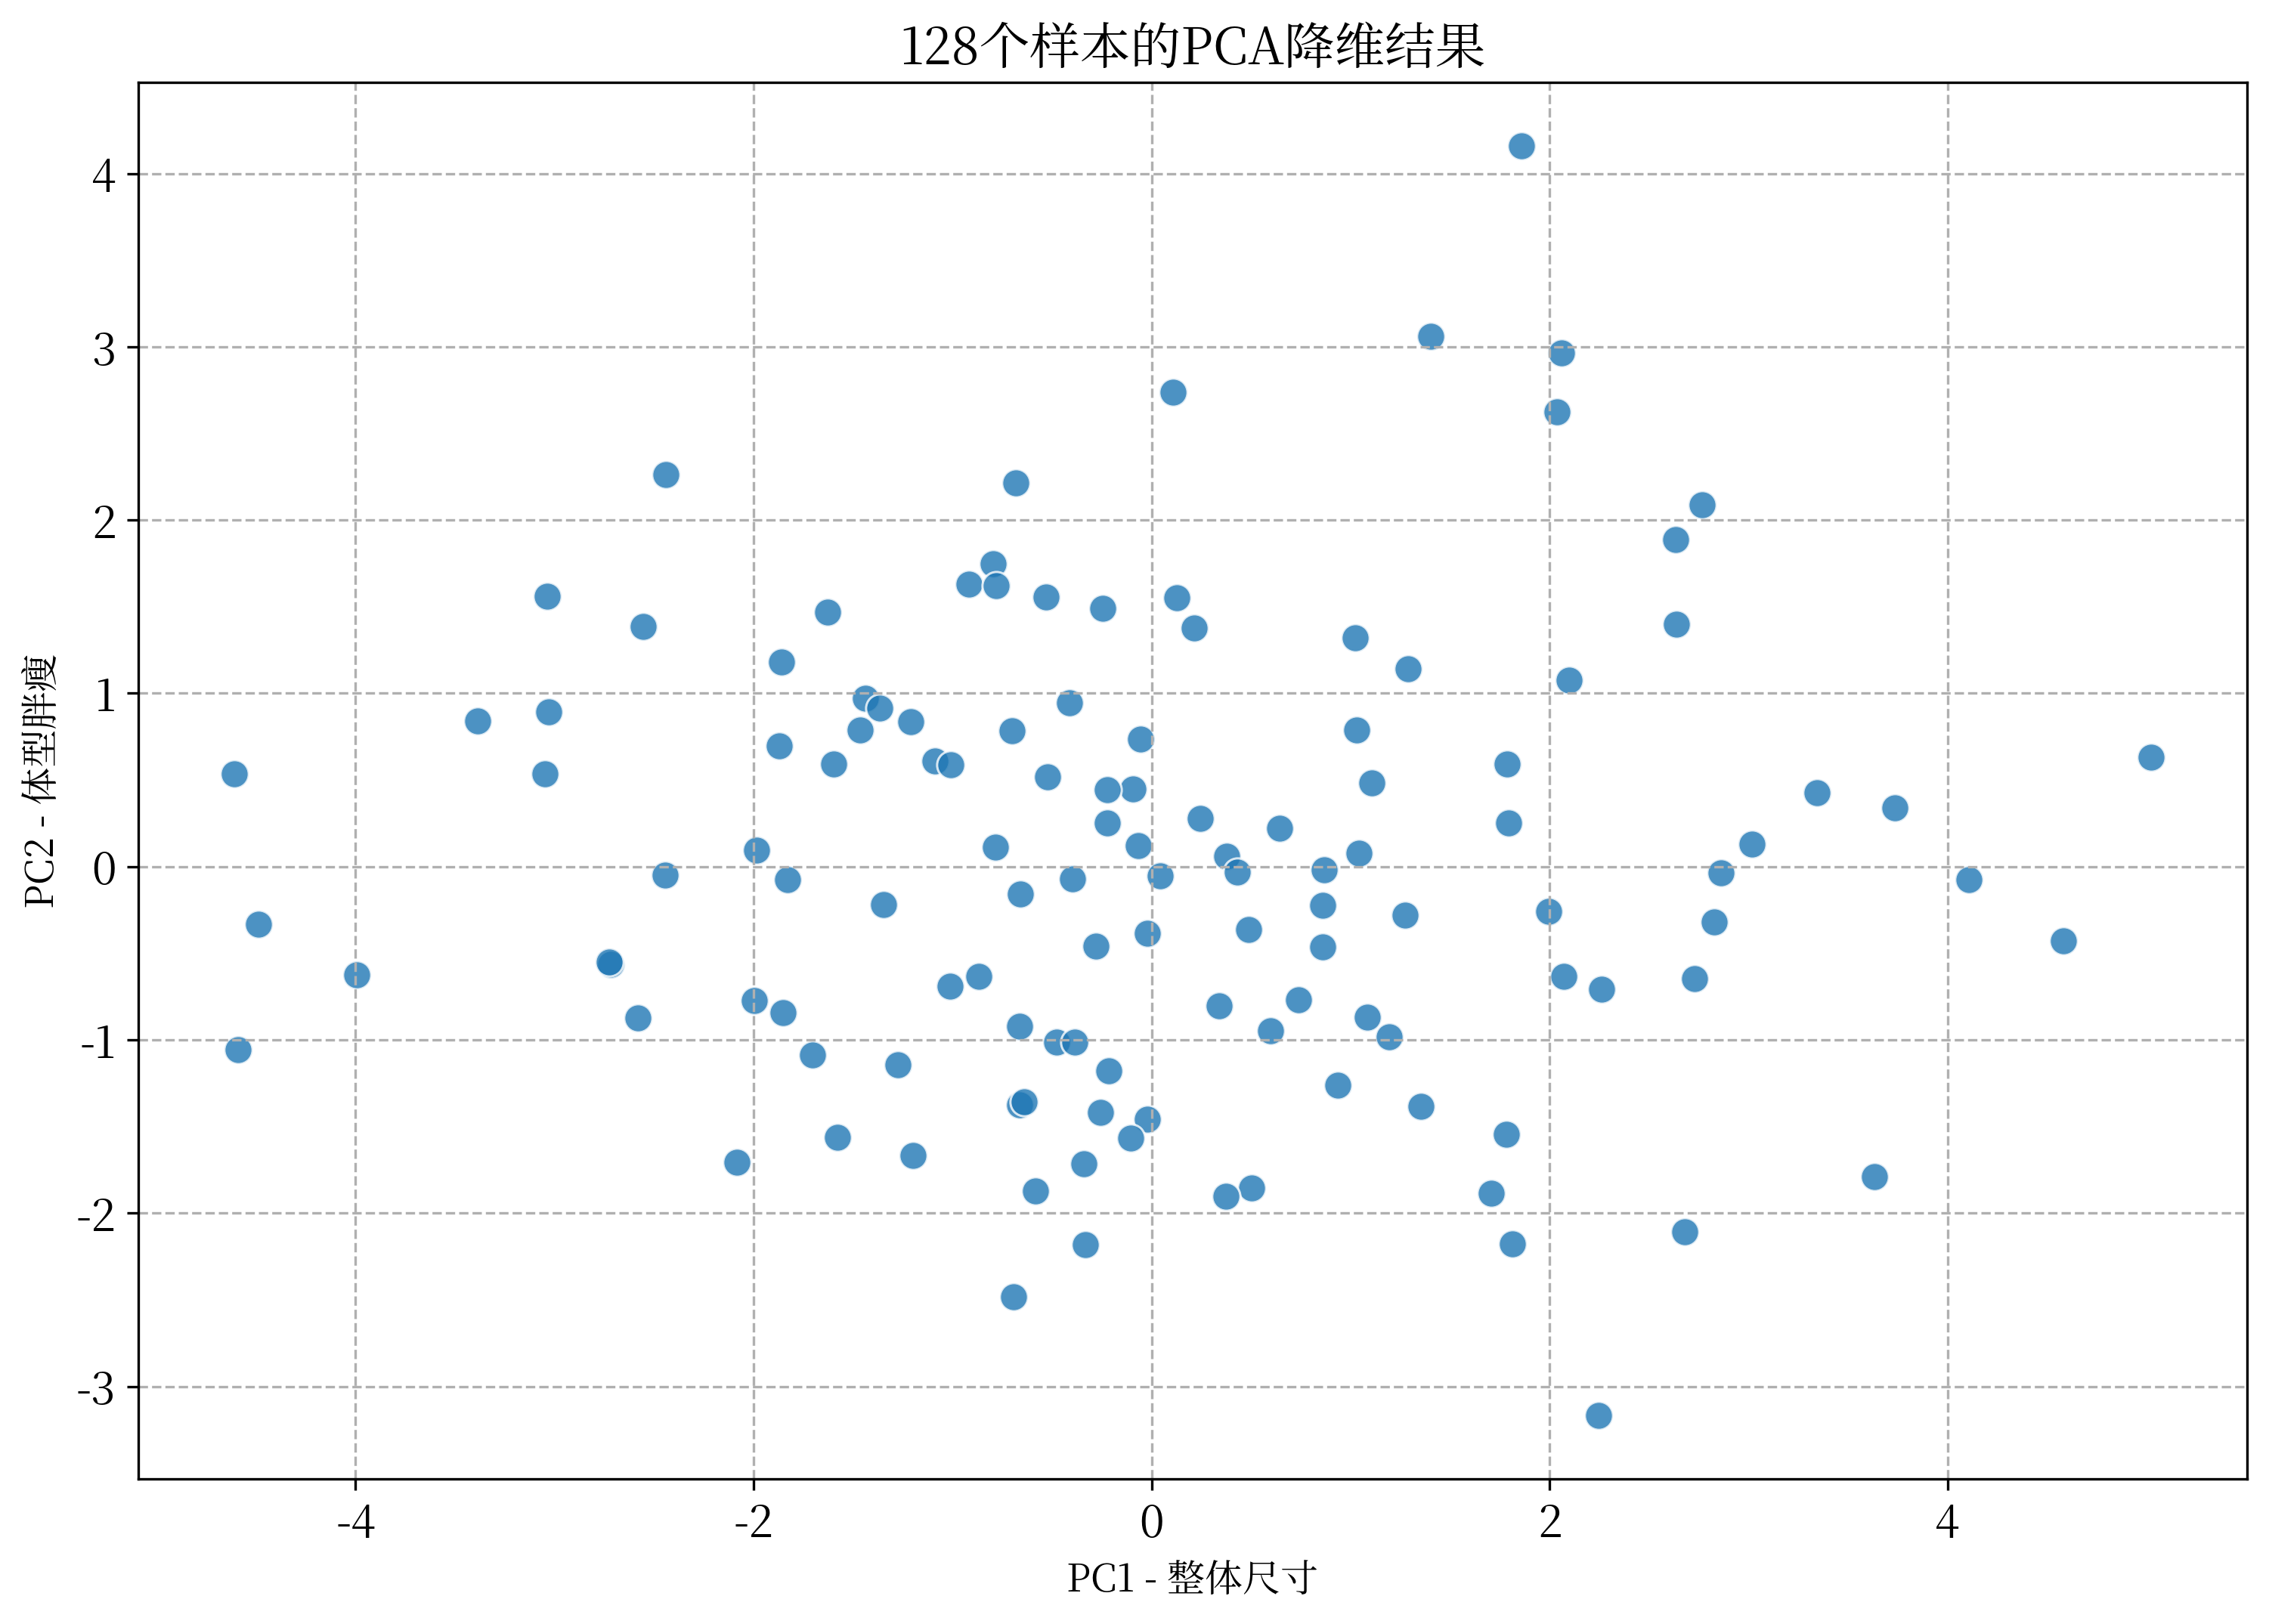
\includegraphics[width=0.4\textwidth]{chapters/主成分分析/images/主成分分析/img-20250829200530.png}
\end{figure}

从这个图中，可以看到我们把多维的评价体系降成了二维，此时数据点围绕着 $(0,0)$ 分布，且可以视作分为四个象限。

有时，在 X 轴方样本变化大，而在 Y 轴方向样本几乎无变化，但如果旋转坐标系，仍然可以进行 PCA 降维。正交变换后在新的坐标系下我们能更清楚看清数据的特点。

\begin{figure} [H]
    \centering
    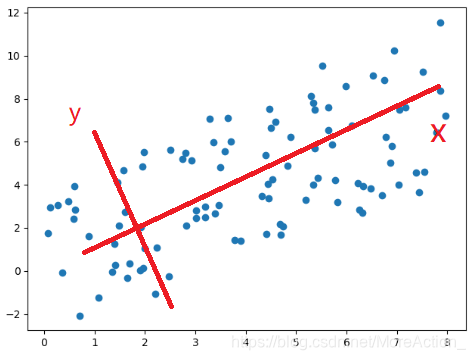
\includegraphics[width=0.4\textwidth]{chapters/主成分分析/images/主成分分析/img-20250830150555.png}
\end{figure}

\section{PCA 绘图}

\begin{definition}[碎石图]
    \begin{enumerate}
        \item 横轴（X轴） ：表示主成分的编号，通常按主成分的重要性从第一个主成分（PC1）到最后一个主成分依次排列。
        \item 纵轴（Y轴） ：表示每个主成分所解释的方差（或特征值），通常表现为每个主成分对应的方差百分比，或直接使用特征值。
    \end{enumerate}
\end{definition}

\begin{figure} [H]
    \centering
    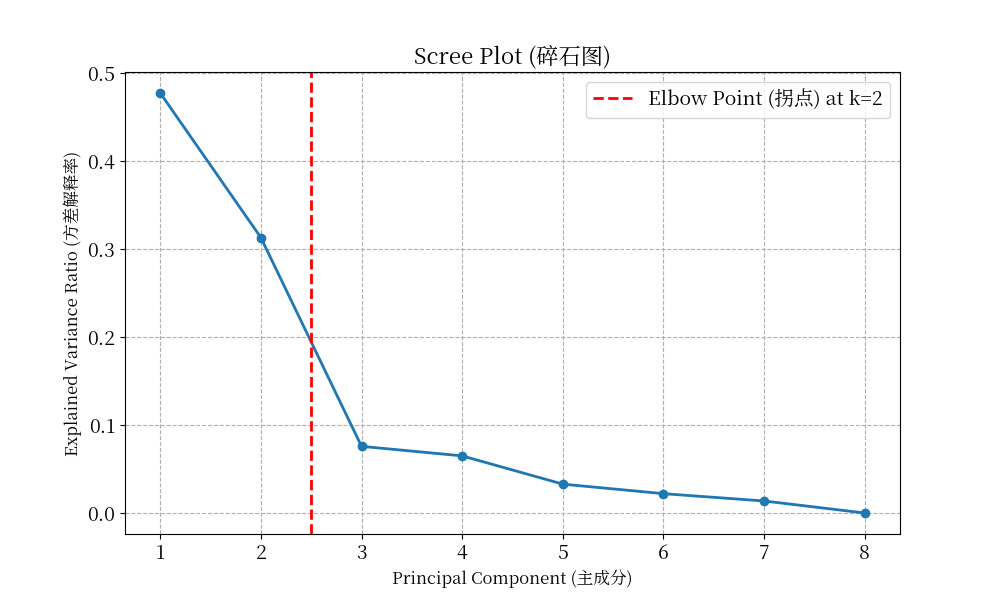
\includegraphics[width=0.7\textwidth]{chapters/主成分分析/images/主成分分析/img-20250902114234.png}
\end{figure}

\begin{definition}[载荷图]
    载荷图显示每个特征对主成分的影响程度。
    \begin{enumerate}
        \item 点/箭头 ：图上的每个点或箭头代表一个原始变量。这些点/箭头的坐标对应于该变量在不同主成分上的载荷值。
        \item 载荷值 ：载荷值的大小反映了原始变量与主成分之间的相关性。载荷值的取值范围通常在-1到1之间。值越接近1或-1，说明该变量与主成分的关系越强；值越接近0，说明该变量与主成分的关系越弱。
    \end{enumerate}
\end{definition}

\begin{tips}
    方向和大小：如果一个变量在某个主成分上的载荷值为正且较大，说明该变量与这个\begin{enumerate}
        \item 主成分正相关，即该变量值越大，主成分值也越大。
        \item 如果载荷值为负且绝对值较大，说明该变量与主成分负相关，即该变量值越大，主成分值越小。
        \item 如果载荷值接近0，说明该变量与主成分几乎没有相关性
    \end{enumerate}
    变量之间的夹角：
    \begin{enumerate}
        \item 如果两个变量在载荷图上的夹角较小，说明这两个变量之间有较强的正相关关系。
        \item 如果夹角接近90度，说明这两个变量之间几乎没有相关性。
        \item 如果夹角接近180度，说明这两个变量之间有较强的负相关关系。
    \end{enumerate}
    主成分的组合解释：通常我们通过观察前两个或前三个主成分的载荷图来解释数据。例如，PC1和PC2组合可能解释了数据中的大部分方差，通过载荷图我们可以看到哪些变量对这两个主成分贡献最大，并尝试从业务角度解释这些主成分的实际意义。
\end{tips}


\begin{definition}[得分图]
    得分图是通过主成分分析（PCA）将高维数据投影到低维空间后，得到的样本在主成分上的得分分布图。得分图可以帮助我们直观地观察样本在主成分空间中的分布情况，识别潜在的聚类结构或异常点。
    \begin{enumerate}
        \item 横轴（X轴） ：通常代表第一个主成分（例如PC1），显示各个样本在这个主成分上的得分。
        \item 纵轴（Y轴） ：通常代表第二个主成分（例如PC2），显示各个样本在这个主成分上的得分。
        \item 点 ：图上的每个点代表一个样本。这些点的坐标对应于该样本在不同主成分上的得分。
    \end{enumerate}
\end{definition}

\begin{definition}[双标图]
    双标图是得分图和载荷图的结合体，呈现在一个图上。
\end{definition}

\begin{figure} [H]
    \centering
    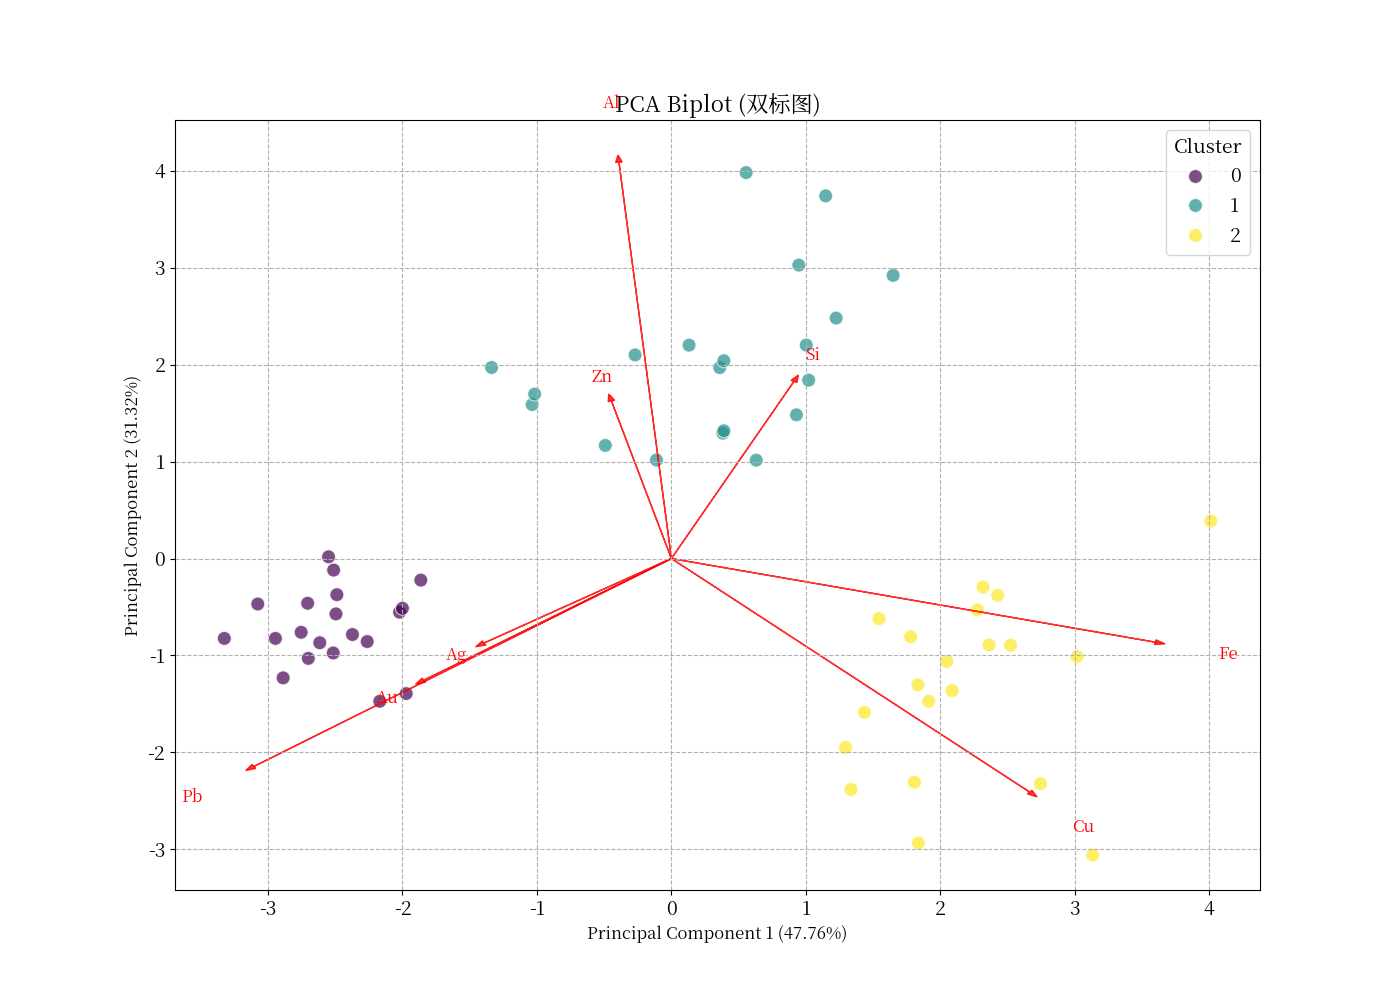
\includegraphics[width=0.7\textwidth]{chapters/主成分分析/images/主成分分析/img-20250902115316.png}
\end{figure}

\section{Kaiser 准则}

\begin{definition}[Kaiser 准则]
    Kaiser准则的逻辑是：如果一个主成分的特征值大于 $1$，那么该主成分解释的方差比单个原始变量解释的方差更多。对于标准化数据，每个原始变量的方差为 $1$，因此，如果某个主成分的特征值小于 $1$，那么这个主成分解释的方差还不如一个原始变量，可能不值得保留。
\end{definition}

\begin{lstlisting}[style=python]
def apply_kaiser_criterion(pca_model: PCA) -> int:
    """应用 Kaiser 准则 (特征值 > 1) 来确定主成分数量"""
    eigenvalues = pca_model.explained_variance_

    print("各主成分的特征值 (Eigenvalues):")
    for i, eig in enumerate(eigenvalues):
        print(f"  PC{i + 1}: {eig:.4f}")

    n_components = np.sum(eigenvalues > 1)
    print(f"\n根据 Kaiser 准则 (特征值 > 1)，推荐保留的主成分数量为: {n_components}")
    return n_components
\end{lstlisting}
